%----------------------------------------------------------------
%
%  File    :  thesis.tex
%
%  Authors :  Keith Andrews, IICM, TU Graz, Austria
%             Manuel Koschuch, FH Campus Wien, Austria
%			  Sebastian Ukleja, FH Campus Wien, Austria
% 
%  Created :  22 Feb 96
% 
%  Changed :  14 Oct 2020
%
%  For suggestions and remarks write to: sebastian.ukleja@fh-campuswien.ac.at
% 
%----------------------------------------------------------------

% --- Setup for the document ------------------------------------

%Class for a book like style:
\documentclass[11pt,a4paper,oneside]{scrbook}
%For a more paper like style use this class instead:
%\documentclass[11pt,a4paper,oneside]{thesis}

%input encoding for windows in utf-8 needed for Ä,Ö,Ü etc..:
\usepackage[utf8]{inputenc}
%input encoding for linux:
%\usepackage[latin1]{inputenc}
%input encoding for mac:
%\usepackage[applemac]{inputenc}

\usepackage[english]{babel}
% for german use this line instead:
%\usepackage[ngerman]{babel}

%needed for font encoding
\usepackage[T1]{fontenc}

%Package for floating figures
\usepackage{float}

% want Arial? uncomment next two lines...
%\usepackage{uarial}
%\renewcommand{\familydefault}{\sfdefault}

% BIBLOGRAPHY
\usepackage{biblatex}
\addbibresource{testBib.bib}

%some formatting packages
\usepackage[bf,sf]{subfigure}
\renewcommand{\subfigtopskip}{0mm}
\renewcommand{\subfigcapmargin}{0mm}

%For better font resolution in pdf files
\usepackage{lmodern}

\usepackage{url}

%\usepackage{latexsym}

\usepackage{geometry} % define pagesize in more detail


\usepackage{colortbl} % define colored backgrounds for tables

\usepackage{biblatex}

\usepackage{courier} %for listings
\usepackage{listings} % nicer code formatting
\lstset{basicstyle=\ttfamily,breaklines=true}

\usepackage{graphicx}
  \pdfcompresslevel=9
  \pdfpageheight=297mm
  \pdfpagewidth=210mm
  \usepackage[         % hyperref should be last package loaded
    pdftex, 		   % needed for pdf compiling, DO NOT compile with LaTeX
    bookmarks,
    bookmarksnumbered,
    linktocpage,
    pdfview={Fit},
    pdfstartview={Fit},
    pdfpagemode=UseOutlines,                 % open bookmarks in Acrobat
  ]{hyperref}
\DeclareGraphicsExtensions{.pdf,.jpg,.png}
\usepackage{bookmark}

\usepackage[title]{appendix}

%paper format
\geometry{a4paper,left=30mm,right=25mm, top=30mm, bottom=30mm}

% --- Settings for header and footer ---------------------------------
\usepackage{scrlayer-scrpage}
\clearscrheadfoot
\pagestyle{scrheadings}
\automark{chapter}

%Left header shows chapter and chapter name, will not display on first chapter page use \ihead*{\leftmark} to show on every page
\ihead{\leftmark} 	
%\ohead*{\rightmark}	%optional right header
\ifoot*{Student}		%left footer shows student name
\ofoot*{\thepage}		%right footer shows pagination
%---------------------------------------------------------------------

%Start of your document beginning with title page
\begin{document}


% --- Main Title Page ------------------------------------------------
\begin{titlepage}
\frontmatter

\begin{picture}(50,50)
\put(-70,40){\hbox{
\includegraphics{images/logo.png}}}
\end{picture}

\vspace*{-5.8cm}

\begin{center}

\vspace{6.2cm}

\hspace*{-1.0cm} {\LARGE \textbf{Web 3.0\\}}
\vspace{0.2cm}
\hspace*{-1.0cm} Definition, Challenges and Opportunities\\

\vspace{2.0cm}

\hspace*{-1.0cm} { \textbf{Bachelor Thesis\\}}

\vspace{0.65cm}

\hspace*{-1.0cm} Submitted in partial fulfillment of the requirements for the degree of \\

\vspace{0.65cm}

\hspace*{-1.0cm} \textbf{Bachelor of Science in Engineering\\}

\vspace{0.65cm}

\hspace*{-1.0cm} to the University of Applied Sciences FH Campus Wien \\
\vspace{0.2cm}
\hspace*{-1.0cm} Bachelor Degree Program: Computer Science and Digital Communications \\

\vspace{1.6cm}

\hspace*{-1.0cm} \textbf{Author:} \\
\vspace{0.2cm}
\hspace*{-1.0cm} Gabriel Hübner \\

\vspace{0.7cm}

\hspace*{-1.0cm} \textbf{Student identification number:}\\
\vspace{0.2cm}
\hspace*{-1.0cm} 2010475105, 01408046\\

\vspace{0.7cm}

\hspace*{-1.0cm} \textbf{Supervisor:} \\
\vspace{0.2cm}
\hspace*{-1.0cm} BSc MSc Leon Freudenthaler \\

\vspace{0.7cm}

% Reviewer if needed
%\hspace*{-1.0cm} \textbf{Reviewer: (optional)} \\
%\vspace{0.2cm}
%\hspace*{-1.0cm} Title first name surname \\


\vspace{1.0cm}

\hspace*{-1.0cm} \textbf{Date:} \\
\vspace{0.2cm}
\hspace*{-1.0cm} dd.mm.yyyy \\

\end{center}
\end{titlepage}

\newpage

\vspace*{16cm}
\setcounter{page}{1}

% --- Declaration of authorship ------------------------------------------
\hspace*{-0.7cm} \underline{Declaration of authorship:}\\\\
I declare that this Bachelor Thesis has been written by myself. I have not used any other than the listed sources, nor have I received any unauthorized help.\\\\
I hereby certify that I have not submitted this Bachelor Thesis in any form (to a reviewer for assessment) either in Austria or abroad.\\\\
Furthermore, I assure that the (printed and electronic) copies I have submitted are identical.
\\\\\\
Date: \hspace{6cm} Signature:\\

% --- English Abstract ----------------------------------------------------
\cleardoublepage
\chapter*{Abstract}
(E.g. ``This thesis investigates...'')

% --- German Abstract ----------------------------------------------------
\cleardoublepage
\chapter*{Kurzfassung}
(Z.B. ``Diese Arbeit untersucht...'')


% --- Abbrevations ----------------------------------------------------
\chapter*{List of Abbreviations}
\vspace{0.65cm}

\begin{table*}[htbp]
		\begin{tabular}{ll}
			
		\end{tabular}
\end{table*}

% --- Key terms ----------------------------------------------------
\newpage
\chapter*{Key Terms}
\vspace{0.65cm}

\begin{itemize}
	\setlength{\itemsep}{0pt}
	\item[] Web3
	\item[] Web 3.0
	\item[] Semantic Web
    \item[] Blockchain
\end{itemize}

% --- Table of contents autogenerated ------------------------------------
\newpage
\setcounter{tocdepth}{3}
\tableofcontents
\thispagestyle{empty}

% --- Begin of Thesis ----------------------------------------------------
\mainmatter
\chapter{Introduction}
\label{chap:intro}

\subsection{Contribution}

\subsection{Relevance}

\subsection{State of the Art}

\subsection{Methodology}

\subsection{Outlook}

\newpage
\chapter{Web 3.0}
The first question, that emerges, when talking about the web 3.0 (also called the Web3), is what it is by definition. There is neither an easy, nor a precise answer to that question, since there are many different definitions of the term. To better understand what the Web 3.0 is and what the term stands for, we can analyse the history of the two previous iterations of the web, the web 1.0 and web 2.0.

\section{History of the Web}
First of, it is important to understand, that the evolution of the web 1.0 to the web 2.0 didn't take place at a concrete time. It was rather a slow progress, where certain websites gradually implemented additional functionalities and technologies, eg. AJAX. \cite{oreilly2007}\\

\textbf{Web 1.0}\\

The first "packet-switched" network, the ARPANET (Advanced Research Project Agency Network), was created in 1969 in the United States. This network connected four Universities and was one of the earliest forms of the internet. To accommodate for an open-architecture network environment Robert Kahn formalised the Transmission Control Protocol/Internet Protocol (TCP/IP), which was then implemented by Ray Tomlinso and Peter Kirstein. In the 1980´s Bob Metcalfe developed Ethernet Technology to connect a number of hosts in Local Area Networks (LANs). Later the Domain Name System (DNS) was invented by Paul Mockapetris to resolve host names into IP addresses. With these protocolls, the basic building blocks of the internet were laid out.\cite{arxiv.org}\\

The "world-wide web" or web for short, has been established by Tim Burners-Lee in late 1989. This were static websites, which allowed users to read information and jump to different sites with the use of hyperlinks. In this sense, the web 1.0 was mostly a "read-only" web. This iteration of the web lasted until roughly 2005, when the web 2.0 was introduced.\cite{hiremath2016}\\
Figure 2.1 depicts a screenshot of the "first website", which was recreated and is hosted on \hyperlink{http://info.cern.ch/hypertext/WWW/TheProject.html}{info.cern.ch}.

\begin{figure}[H]
	\centering
		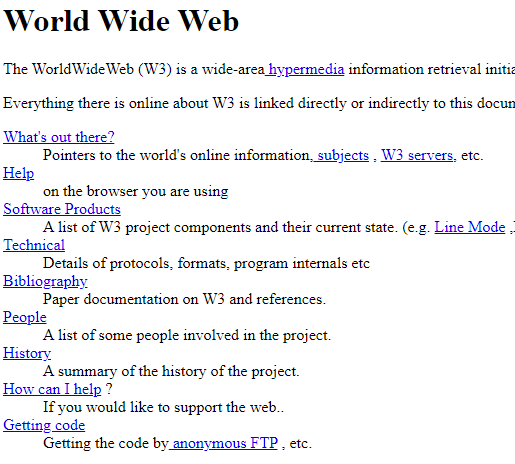
\includegraphics[width=12cm,keepaspectratio]{images/first_website.png}
	\caption{First Website}
	\label{fig:first-website}
\end{figure}

\textbf{Web 2.0}\\\\
The term for the web 2.0 was first coined in 2004 by Dale Dougherty and Craig Cline in a conference with Tim O'Reilly. The key difference to the first iteration of the web, is that the second web allows read and write access instead of mostly read access. This could also be described as the first "dynamic" web, in contrast to the "static" web 1.0. Through "social-media" websites, "blogs", etc. users can generate content on a website, this leads to the terms "participative" web and "people-centric" web, for the web 2.0. \cite{hiremath2016}\\

Tim O'Reilly describes the web 2.0 as network with "rich user experiences", which are provided by websites from major corporations, such as the google search engine. One of the key components is AJAX, which is composed of several technologies, such as XHTML and CSS to represent the data on website, the Dosument Object Model, XML and XSLT, XMLHttpRequest for asynchronos data retrieval and JavaScript to bind everything together.\cite{oreilly2007}\\

Nowadays there are of course several other or newer technologies and further developments of the web 2.0, however the core-concepts remain roughly the same.\\

This chapter should provide a general understanding of the history of the web, as well as a demarcation of the web 2.0 to the web 3.0.
The next chapter will introduce a definition, as well as new technologies of the web 3.0. \\

\section{Definition of Web 3.0}
Defining web 3.0 is a challenging task, because there are many different definitions, which can be used. The availability of scientific papers in regard of the definition of web 3.0 is relatively sparse, therefore online sources have been used.\\
As of now there is no concise definition for the third generation of the web to be found, since it is still being defined and evolving. \cite{techtarget}\\

When searching for the definition of the web 3.0, it is often also called the semantic web, the transcendent web and the web of things. In this paper it will be described as the web 3.0 or the new generation of the web. In contrast to the web 2.0, where data is created by humans, it is described as a web, where data is created by computers / machines. \cite{definingweb3}\\

As a side note, the term "semantic web" often seems confusing, because it is sometimes used as a synonym for the web 3.0. This term was coined by Tim Berners-Lee, who predicted the possibility of computers to exchange semantic data.\cite{newmedia}
In this paper, the "semantic web" is not equal to the web 3.0, it is rather a technology that is incorporated into it.\cite{avast}\\
The metadata (semantic data) in the semantic web, is data which describes data, so that it can be used/categorised by a computer. It can be used to optimize search engines, as well as a variety of other fields. \cite{CLARKE201279}\\

Carly Burdova from avast describes the web 3.0 as follows: \begin{quote}
    "Web 3.0, also known as Web3, is the third generation of the World Wide Web. Web 3.0 is meant to be decentralized, open to everyone (with a bottom-up design), and built on top of blockchain technologies and developments in the Semantic Web, which describes the web as a network of meaningfully linked data."\cite{avast}
\end{quote}

She also states the features that the new generation of the web should encompass. These features are decentralization, artificial intelligence, ubiquity and semantic web interactivity.\cite{avast}\\

A further feature of the web 3.0 is to enhance security and the privacy of users.\cite{connected2022}\\

Another term, which frequently comes up, when searching for definitions of the web 3.0 is the "3d web", which refers to the use of 3d graphics in the web. This could mean, that the web could be enhanced into an immersive experience with the use of augmented and virtual reality.\cite{education2011}\\

A simple architecture for the web 3.0 could look as depicted in figure XXXX. The key difference is, that instead of a database, as currently in the web 2.0 a blockchain is used. In this case it is the widely popular etherum blockchain.\cite{newstack}

%\begin{figure}[H]
%	\centering
%		\includegraphics[width=12cm,keepaspectratio]{images/web3_architecture}
%	\caption{Web 3.0 Simple Architecture [source: author]}
%	\label{fig:web3-architekture}
%\end{figure}


From these definitions, it should be easy to see, that the web 3.0 is still a work in progress.\\
To better understand what the web 3.0 is, it is necessary, to look at the technologies, which enable it. In the next chapter the underlying technologies of the web3.0 will be presented.


\newpage
\section{Technologies}
There are several technologies, which are used in the new generation of the web. Many of those have already been named in chapter 2.2.1. In this section the core concepts of enabling technologies of the web 3.0 will be presented.\\

\subsection{Blockchain technology}
One major part of the web 3.0 is the Blockchain technology. This enables the decentralized part of the new generation of the web. The blockchain technology has gotten much attention in recent years, since the rise of cryptocurrency. The most popular implementation of a Blockchain is Bitcoin, which, at the time of writing this paper has a market capitalization of over 420 Billion Dollars, as stated on \href{https://www.coinbase.com/explore}{coinbase.com}. Another popular blockchain technology is ethereum, with a market capitalisation of over 180 Billion Dollars. In this paper, ethereum will be the distributed-ledger technology of choice, since it has very good documentation, is constantly improved and has a large community behind it.\\

Blockchain falls into a category of a distributed ledger technology. This technology can fulfill some of the goals of web 3.0, because of its properties of a decentralised network, anonymity, persistency and auditability. A blockchain consits, as the name already suggests, of a sequence of blocks, where each block can hold a certain set of data. In the field of cryptocurrency, this data encompasses all the transactions that have been made with the currency.  \cite{blockchaingeneral}

\begin{figure}[H]
	\centering
		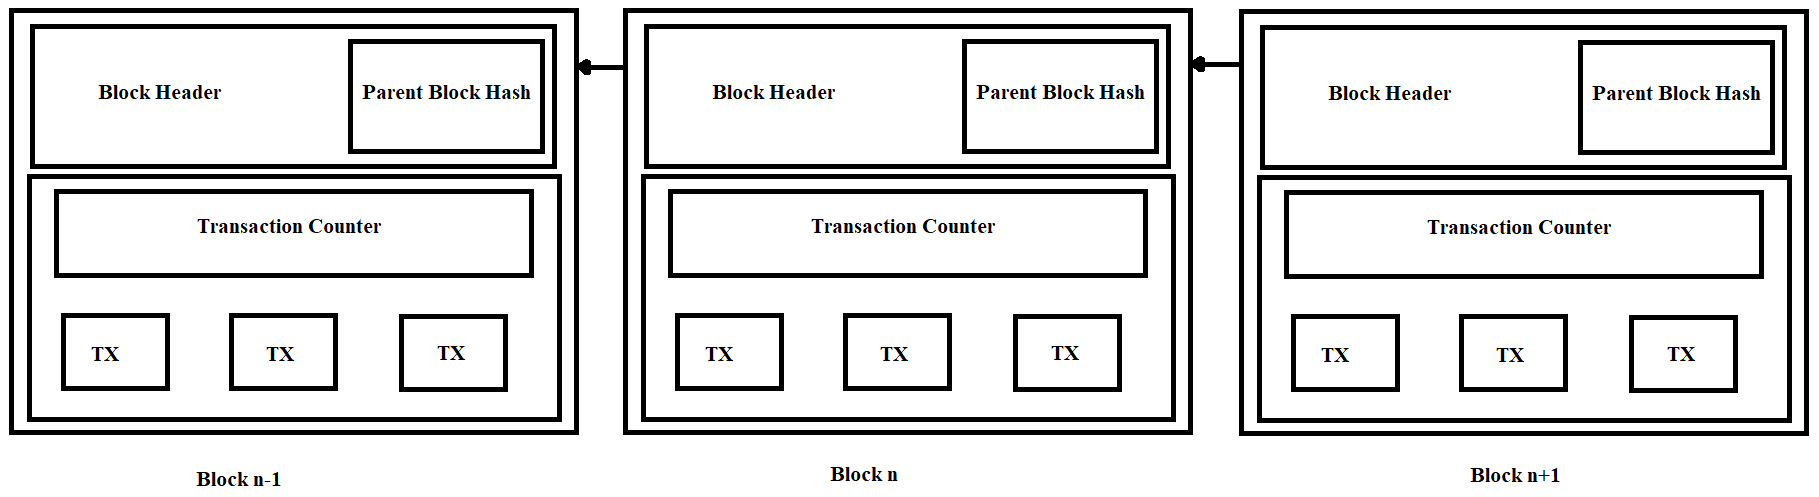
\includegraphics[width=15cm,keepaspectratio]{images/blockchain architecture.png}
	\caption{Blockchain Architecture}
	\label{fig:blockchain-architecture}
\end{figure}

The blocks of a blockchain differ with the specific implementation of a blockchain, however some basic elements are always roughly the same. In a blockchain each block has a reference to its parent/previous block, where the reference is in form of a cryptographic hash of a previous block, which is stored in the block header. A cryptographic hash is a sort of algorithm, that transform a set of data into a string, that is always the same length. The reference to the previous block is always there except for the first block in a blockchain (also called the genesis-block). \\
In Figure 2.2 an example of a blockchain architecture is depicted. The block header usually contains a version number, a timestamp, a field for the hashed value of all transactions contained in the block, a nonce - which is important for a security aspect of the blockchain as well as creating new blocks, a field for the threshold of a valid block hash and as already explained, the parent block hash, which links the preceding block.\\
The decentralized part of the blockchain is then made possible by people who provide their own network bandwidth and computational power to the network. These people are called miners and represent the nodes of a network. The miners are responsible for adding new blocks to the blockchain, in the case of cryptocurrency, they are therefore responsible for the validation of transactions in the network. As a reward for the participation of miners, they get a certain amount of the cryptocurrency e.g. Ethereum, whenever a new block is created. The process of validating the blockchain is called the consensus process, in a public blockchain, each user can participate in this process.\\
The first, well known consensus strategy, which is also used in the Bitcoin network is the Proof of Work (PoW) strategy. This requires complex mathematical calculations to be done, which also creates a number of problems e.g. energy cost, that will be addressed in chapter 3.\\
Another strategy is the Proof of Stake (PoS) strategy, which addresses some of he problems of PoW, but introduces new problems of their own.\cite{blockchaingeneral}\\

\subsubsection{Proof of Work}
As already mentioned in the previous chapter, PoW is a conses mechanism/system, which is used in many blockchains. It was first introduced in the Bitcoin blockchain. The peers or miners in a network can so to speak vote with their respective computing power, by solving mathematical problems and then creating the appropriate blocks of the blockchain. The miners have to find the correct nonce of value of a block. When this value is then hashed with additional block parameters the value of the resulting hash has to be smaller then the momentary target value. Once the correct nonce is found, the block is created and forwarded on the network layer to all the peers in the network. This block is then validated by the other peers in the network.\cite{pow2016}

\subsubsection{Proof of Stake}
As already mentioned, the PoW mechanism has a high demand for energy among other shortcomings, which is why the PoS mechanism was developed.\\  
PoS is meant to reduce the computational power needed to solve problems, as is the case with PoW. Instead of every peer in a network competeing to solve the next block in a blockchain, to get the mining reward, a leader is selected based on their stakes e.g. in cryptocurrency that would be the number of coins in possession. This promises lower energy cuonsumption, as well as a faster speed, at which transactions are confirmed.\cite{pos}\\\\


Two further technologies, which are important and often found in combination with the term web 3.0 are smart contracts and DApps (Decentralized Apps). These will be presented in the next chapters.

\newpage

\subsection{Smart contracts}
The term "smart contract" was frist coined in 1994 by Nick Szabo. He already foresaw a marketplace in the digital world, built on these processes/contracts.\\
The main idea behind smart contracts is to create a digital contract, without the need of a middle-man e.g. a lawyer, who ensures that the contract is not changed after all involved parties have agreed to the terms of said contract.\\
The clauses written in  a smart contract will be automatically executed, when certain conditions are met. This applies also if one of the parties involved in a smart contract breaches a clause, then said party will be automatically punished. In the case of cryptocurrency, this means, that the party breaching the contract will be deducted a certain amount of coins, which is specified in the smart contract.\\
This contracts are pieces of code, which run directly on a blockchain. In the case of the ethereum blockchain, as described on \href{https://ethereum.org/en/developers/docs/smart-contracts/}{ethereum.org} they are a type of an ethereum account themselves. This means, that the contract itself can be the target of a transaction and has an account balance. They are not controlled by a user, they rather run automatic, and execute the code according to their programming. An example for a smart contracts would be a vending machine, which operates as follows:
\begin{itemize}
    \item A product is selected
    \item The vending machine displays the cost of the selected product
    \item The amount to buy the product is inserted into the vending machine
    \item The program on the vending machine verifies that the inserted amount matches the cost of the product
    \item The selected product is dispensed
\end{itemize}
This example should show, that the product is only dispensed after all requirements have been met. Just like a vending machine a smart contract automatically checks, if all requirements have been met and then executes a specified part of the code.
\cite{ethereumsmartcontracts}\cite{ethereumsmartcontractsgeneral}\cite{smartcontracts2019}

\subsection{DApps}
Decentralised applications are built on decentralised networks. They work, by combining a smart contract and a user interface. This means theta the business logic or the backend code of a DApp runs on the decentralised network and the frontend runs on the client. They have a certain set of characteristics, which can be described as follows:
\begin{itemize}
    \item The are decentralized, which mean that they run on a peer-to-peer network
    \item They are deterministic, that means that they always perform the same functions, regardless of the environment they are run in
    \item They are Turing complete, which means, that if enough resources are provided, they can perform any action
    \item They are isolated, that means that an error won't disturb the normal functioning of the network they are run in
\end{itemize}\cite{ethereumddapps}
\newpage

\section{The semantic web}

%TODO - lead into next part

%The paper "Make Web3.0 Connected" \cite{connected2022} defines three infrastructural enablers for %the web 3.0:
%\begin{enumerate}
%    \item Blockchains, through this technology verifiable computing can be supported
%    \item Federated / centralised platforms, these should be able to publish verifiable states, %because some functionalities are difficult to implement on a blockchain
%    \item A secure platform, which serves as a connection between blockchains and platforms
%\end{enumerate}




\newpage
\chapter{Challenges of the Web 3.0}

\newpage
\chapter{Opportunities of the Web 3.0}

\newpage
\chapter{Related Work}

\newpage
\chapter{Conclusion}

\newpage
\chapter{Future work}

\newpage
\chapter{Summary}

\newpage

% --- Bibliography ------------------------------------------------------

%IEEE Citation [1]
%\bibliographystyle{IEEEtran}
%for alphanumeric citation eg.: [ABC19]
%\bibliographystyle{alpha}

% List references I definitely want in the bibliography,
% regardless of whether or not I cite them in the thesis.

\newpage
\addcontentsline{toc}{chapter}{Bibliography}
\printbibliography
\newpage

% --- List of Figures ----------------------------------------------------

\addcontentsline{toc}{chapter}{List of Figures}
\listoffigures


% --- List of Tables -----------------------------------------------------

\newpage
\addcontentsline{toc}{chapter}{List of Tables}
\listoftables

% --- Appendix A -----------------------------------------------------

\backmatter
\appendix
\begin{appendices}
\chapter{Appendix}

(Hier können Schaltpläne, Programme usw. eingefügt werden.)

\clearpage
\end{appendices}

\end{document}
